\documentclass[a4paper, 10pt]{article}
\usepackage[a4paper,left=3cm,right=2cm,top=2.0cm,bottom=1.5cm]{geometry}
\usepackage{hyperref}

\hypersetup{
    colorlinks=true,
    linkcolor=black,
    urlcolor=blue,
}

\urlstyle{same}

\usepackage[utf8]{inputenc} % Change according your file encoding
\usepackage{graphicx}
%\usepackage[demo]{graphicx}
\usepackage{url}

\usepackage{float}
\usepackage{amsmath}
\usepackage{xcolor}
\usepackage{todonotes}
\usepackage{algorithm}
\usepackage{algpseudocode}

\usepackage{listings}

\definecolor{backcolour}{rgb}{0.95,0.95,0.92}

\lstdefinestyle{mystyle}{
    backgroundcolor=\color{backcolour},  
    breakatwhitespace=false,         
    basicstyle=\scriptsize,
    breaklines=true,                 
    captionpos=b,                    
    keepspaces=true,                 
    showspaces=false,                
    showstringspaces=false,
    showtabs=false,                  
    tabsize=2,
    frame=single
}



\lstset{style=mystyle}

%opening
\title{Algorithmic Methods for Mathematical Models\\Course Project}
\author{Ignacio Encinas Rubio, Adrián Jimenez González}
\date{\normalsize\today{}}

\begin{document}

\maketitle

\tableofcontents

\clearpage

\section{Problem statement}
In this section we'll state the inputs, outputs, modelling elements and objective function.

The problem can be summarized into the following requirements:

\begin{enumerate}
    \item Each contestant will play exactly once against each of the other contestants.
    \item Each round will consist of $\frac{n-1}{2}$ matches.
    \item Players will play 50\% of their games as white, 50\% will be played as black.
\end{enumerate}


\subsection{Input}
\begin{itemize}
    \item $n$ is the number of players that will participate in the tournament.
    \item $p_{n \times n}$ is the matrix of points. $p_{ij}$ is the number of points assigned by player $i$ to round $j$.
\end{itemize}

\subsection{Definitions}
We've defined the following sets in order to model the problem:

\begin{itemize}
    \item $P$ is the set of players participating in the tournament. $|P| = n$
    \item Rounds is the number of rounds. In this case it is equal to $|P|$.
    \item $M(x, y)$  is the set of matches played among \textit{x} and \textit{y}.
    \item $F(r)$ is the set of free players at round $r$.
    \item $W(p)$ is the set of matches played by player \textit{p} as white.
    \item $B(p)$ is the set of matches played by player \textit{p} as black.
    \item $R(r)$  is the set of matches played at round \textit{r}.
    \item $G(p,r)$ is the set of games played by player $p$ at round $r$.
\end{itemize}

Thus, the score of a schedule can be computed as followed:

\begin{equation}
    \text{Score} = \sum_{j = 1}^{\text{Rounds}} \sum_{i \in F(r)}  p_{ij}
    \label{objfunc}
\end{equation}


Our goal is to maximize this score.






\subsection{Output}
The output will be an optimal schedule $s$ that maximizes the score. It will contain the matches to be carried out in every round of the tournament.

\clearpage

\section{Integer Linear Programming Model}
Every set will be built from a boolean multidimensional array. \textit{matches}$[w][b][r]$ will be 1 whenever player $w$\footnote{Player with the white pieces} plays player $b$\footnote{Player with the black pieces} in round $r$, and 0 otherwise.


For clarity's sake we'll explicitly state these constructions:

\begin{align*}
    M(x, y)   &= \{ \{x, y, r\} &|& \ \text{matches}[x][y][r] = 1 \lor \text{matches}[y][x][r] = 1   &\forall &r \in [1, Rounds]\}\\
    F(r)      &= \{ p           &|& \ \text{matches}[p][o][r] = 0 \land \text{matches}[o][p][r] = 0  &\forall &o \in [1, n]\}\\
    W(p)      &= \{ \{p, b, r\} &|& \ \text{matches}[p][b][r] = 1                                    &\forall &r \in [1, Rounds], b \in [1, n]\}\\
    B(p)      &= \{ \{w, p, r\} &|& \ \text{matches}[w][p][r] = 1                                    &\forall &r \in [1, Rounds], w \in [1, n]\}\\
    R(r)      &= \{ \{w, b, r\} &|& \ \text{matches}[w][b][r] = 1                                    &\forall &w, b \in [1, n]\}\\
    G(p, r)   &= \{ \{o, p, r\} &|& \ \text{matches}[p][o][r] = 1  \lor \text{matches}[o][p][r] = 1  &\forall &o \in [1, n]\}\\
\end{align*}

The objective function was already described by Eq. \ref{objfunc}

\subsection{Constraints}

\begin{equation}
    \label{playwitheachother}
    |M(x,y)| = 1 \quad \forall x,y \in P \ | \  x \neq y
\end{equation}

Eq. \ref{playwitheachother} ensures ``each contestant will play exactly once against each other of the contestants''.


\begin{equation}
    \label{1gameperround}
    |G(p,r)| \leq 1 \quad \forall p \in P, r \in [1, \ \text{Rounds}] 
\end{equation}
Eq. \ref{1gameperround} ensures that a player plays up to 1 game per round.

\begin{equation}
    \label{matchesperround}
    |R(r)| = \frac{n-1}{2}  \quad \forall r \in [1,\ \text{Rounds}] 
\end{equation}
Eq. \ref{matchesperround} ensures that ``the number of games that are played simultaneously at each slot is always $\frac{n-1}{2}$''

\begin{equation}
    \label{fairness}
    |W(p)| = \frac{n-1}{2} \quad \forall r \in [1, \ \text{Rounds}], \forall p \in P
\end{equation}

Eq. \ref{fairness} ensures that ``a contestant should play black as many whites as white'', 
given that Eq. \ref{playwitheachother} ensures that $|\text{Games}(p)| = n - 1$ and $|\text{Games}(p)| = |W(p)| + |B(p)|$  

\subsection{Redundant constraints}
\label{subsec:redundant}


\begin{minipage}{0.45\linewidth}
\begin{equation}
    \label{noselfplay}
    |M(x,x)| = 0 \quad \forall x \in P 
\end{equation}
Eq. \ref{noselfplay} ensures that a player can't play with himself. 

\begin{equation}
    \label{blackfairness}
    |B(p)| = \frac{n-1}{2} \quad \forall r \in [1, \ \text{Rounds}], \forall p \in P
\end{equation}

    While developing the model, we removed some redundant constraints such as the one described by Eq. \ref{noselfplay}. Initial testing suggested that the redundant ILP model could be faster in some cases, but further testing indicated otherwise. Results shown in Figure \ref{figilp}
\end{minipage}
\begin{minipage}{0.49\linewidth}
\begin{figure}[H]
    \centering
    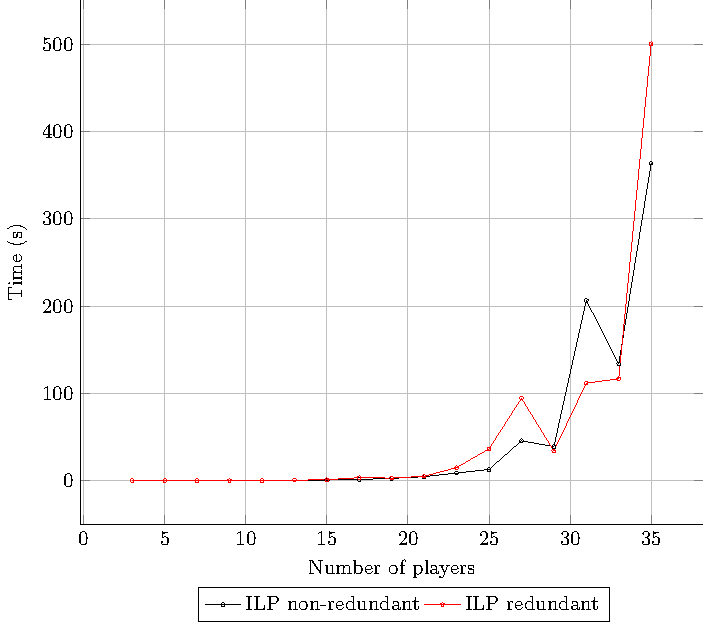
\includegraphics[width=\linewidth]{plots/time_per_instance.pdf}
    \caption{ILP runtime w.r.t the number of players}
    \label{figilp}
\end{figure}
\end{minipage}


\clearpage

\section{Meta-heuristics}

As a solution must exist no matter which player rests in a given day, we will focus on assigning a rest day for every player $p$. This information is enough for calculating our objective function, performing local search and GRASP. After all this, we will determine the pairings for the whole tournament.

\subsection{Constructive}

The greedy cost function is the points that a player $p$ assigns to resting on day $d$. As we want to maximize this, we will sort the available players in descending order and pick the one with highest value.

\begin{equation}
  \label{eq:greedy-cost}
  q(c,day)= c.points\_per\_day[day]
\end{equation}
Eq. \ref{eq:greedy-cost} is used as greedy cost function to take who rests.

\begin{algorithm}
	\caption{Greedy algorithm} 
	\begin{algorithmic}[1]
	  \State Players $\leftarrow$ Set of Players
	  \State rests $\leftarrow$ \{\}
	    \For {day in 0..days}
	      \State playersToRest $\leftarrow$ filter Players(p) $|$ p.hasNotRested
        \State sortedPlayers $\leftarrow$ sort playersToRest(p) by q(p,day) (DESC) 
	      \State select p $\in$ sortedPlayers[0]
	      \State rests[day]\ $\leftarrow$\ p
	    \EndFor
	\end{algorithmic} 
\end{algorithm}


\subsection{Local search}

In the local search phase we evaluate if swapping the players that rest in two given days increases our objective function\footnote{For simplicity, we initialize the best\_swap so that the local search doesn't change the solution if we found no improvement}.

\begin{algorithm}
	\caption{Local Search} 
	\begin{algorithmic}[1]
    \For {i in 0..days}
    \State best\_swap\_points $\leftarrow$ 0
    \State best\_swap $\leftarrow$ i
      \For {j in 0..days}
        \State change = EvaluateRestSwap(i,j)
        \If{change $>$ best\_swap\_points}
          \State best\_swap\_points $\leftarrow$ change
          \State best\_swap $\leftarrow$ j
        \EndIf
      \EndFor
      \State rests[i] $\leftrightarrow$ rests[best\_swap]
		\EndFor
	\end{algorithmic} 
\end{algorithm}

We can repeat this procedure iteratively until the local search provides no further improvement just by adding an outer loop.


\clearpage
\subsection{GRASP}

In the GRASP we randomize the selection of the player in descending order by points, according to a RCL calculated by $\alpha$ as shown in Algorithm \ref{rcl}.


\begin{algorithm}
    \caption{constructRCL(day)} 
    \label{rcl}
    \begin{algorithmic}[1]
	\State $q_{max} \leftarrow $ sortedPlayers.first().points[d]
	\State $q_{min} \leftarrow$ sortedPlayers.last().points[d]
	\State $RCL_{max}$ $\leftarrow$ $\{p \in sortedPlayers\ |\ p.points[d] >= q_{max} - \alpha \cdot (q_{max} - q_{min})\}$
    \end{algorithmic} 
\end{algorithm}




\begin{algorithm}
	\caption{GRASP} 
	\begin{algorithmic}[1]
	  \State rests $\leftarrow$ \{\}
	    \For {day in 0..days}
	      \State RCL $\leftarrow$ constructRCL(day)
	      \State select p $\in$ RCL randomly
	      \State rests[day]\ $\leftarrow$\ p
	    \EndFor
	\end{algorithmic} 
\end{algorithm}

Our stopping criteria combines the number of iterations since the last incumbent update and a fixed maximum number of iterations.


\subsubsection{Parameter tuning} 

For tuning $\alpha$, we have compare GRASP's objective function with the optimal solution for each of the instances. Then, for each $\alpha$ we calculate the arithmetic mean error. 

Figure \ref{fig:error} shows the mean error of every $\alpha$ we have tested against instances \{0\dots31\}. Two separate lines are plotted for $\alpha_i = 0 + i \cdot 0.1$ and $\alpha_i' = 0 + i \cdot 0.01$. Results show that many values for alpha give good results. We decided to keep the smallest alpha that gives the minimizes the mean error, so $\alpha = 0.19$ is the chosen value after tuning.

\begin{figure}[H]
    \centering
    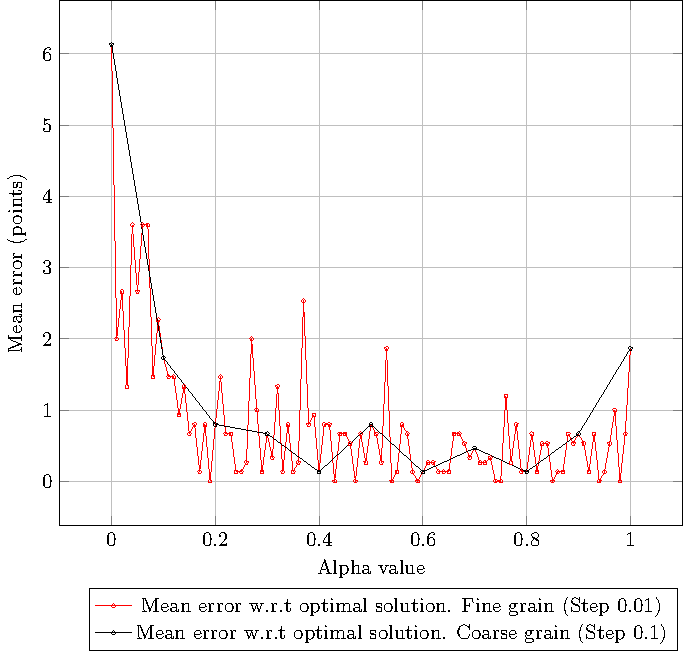
\includegraphics[width=0.7\linewidth]{plots/error.pdf}
    \caption{Mean error w.r.t alpha}
    \label{fig:error}
\end{figure}

\clearpage

\section{Results}

\subsection{Time}

Figure \ref{fig:time} shows the runtime needed for the different models and solvers. Section \ref{subsec:redundant} introduced the redundant and non-redundant ILP models. ILP rest corresponds to the ILP model that just computes the optimal rest day for each player, without obtaining a valid tournament schedule. 

\begin{figure}[H]
    \centering
    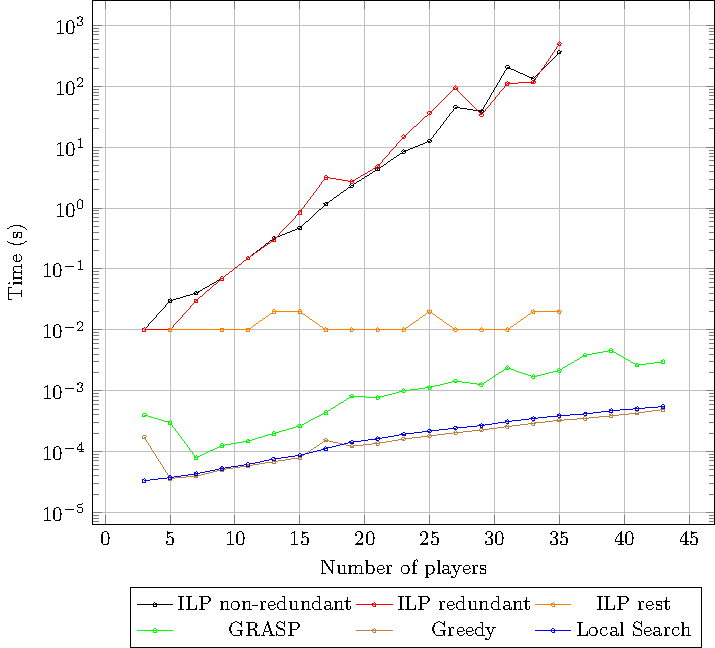
\includegraphics[width=\linewidth]{plots/times.pdf}
    \caption{Runtime for the different ILP models and (meta)heuristic based solvers}
    \label{fig:time}
\end{figure}
Our motivation for testing this simpler ILP model is that while solving the assignment we realized that the hardest part of it was actually getting a valid tournament schedule, not optimizing the objective function. Then, we started wondering whether the CPLEX time cost was spent optimizing the objective function or not. 

Results indicate that our minimal CPLEX model is very fast, and we could combine its output with a tournament schedule maker (see Section \ref{sec:schedule}) to obtain the optimal solution several orders of magnitude faster than the complete CPLEX model while maintaining optimality, in constrast to heuristic-based solvers. For large instances the simple ILP model is even faster than our GRASP implementation\footnote{Of course if the stop criteria plays a great role in the GRASP runtime, and it could be greatly reduced if we're willing to tolerate worse solutions}. 


\clearpage


\clearpage
\subsection{Objective function}

Figure \ref{fig:objfunc} shows the value of the objective function obtained for each of the implementations: ILP, Greedy, Local Search and GRASP. 


\begin{figure}[H]
    \centering
    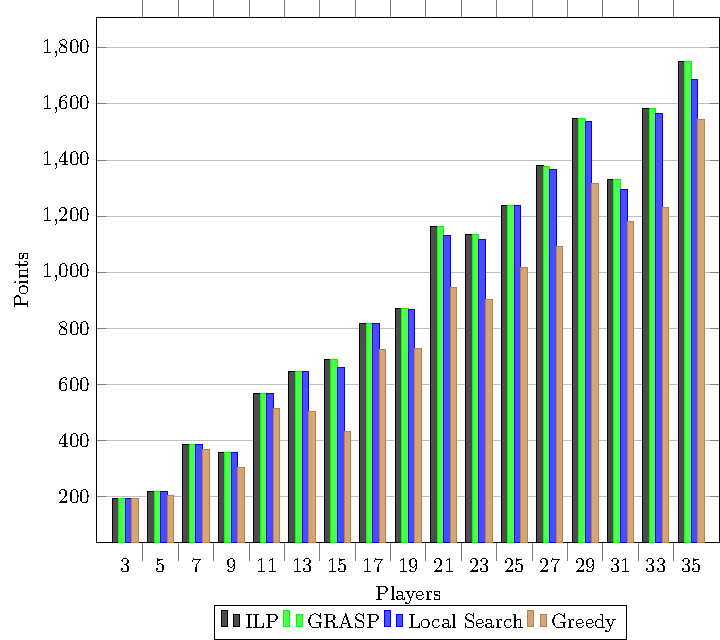
\includegraphics[width=\linewidth]{plots/solutions.pdf}
    \caption{Objective function value per instance and solver}
    \label{fig:objfunc}
\end{figure}

Naturally, greedy offers the worst solution for every instance, while taking practically the same time as Greedy + Local Search. Then, we can conclude that the basic Greedy method shouldn't be used in any case.

Local Search offers great improvement for some instances, but in the majority of the cases it offers a poor solution compared with the optimal one.

GRASP commonly reachs the optimal solution. It obviously does not find it every time but if we're not too concerned with optimality is a great improvement over Local Search.


\clearpage
\section{Schedule construction}
\label{sec:schedule}

When solving the assignment we assumed that the schedule construction would be trivial, and tried to construct it while optimizing the objective function. After many fruitless efforts, we gave up on the idea and decided to make our greedy solver just compute the rest day for each player. This is enough information to compute the objective function, as the actual pairings don't affect it.

We believe that the solution to this part of the assignment should have been provided to us, as it is much more difficult that the actual assignment and has nothing to do with the subject's contents. Even more so considering this was completely accidental.


Just for completeness we will briefly explain our solution and our thought process:

\begin{enumerate}
    \item The problem with making the pairings are the rest days
    \item If there were no rest days and we had an even number of players, obtaining a valid pairing is relatively simple
\end{enumerate}

Then, our solution involves adding every day an extra invalid match for our players. This match can be a match against themselves or against an extra ``fake'' player. After doing this, we have what we wanted: a tournament schedule. The problem with this schedule is that it doesn't take into account our objective function and contains invalid matches, so for the moment it remains useless for us.


\subsection{Solution}
The trick is that we can use this template schedule to construct our desired schedule. The procedure is the following:

Our template schedule $t$ will contain an invalid match each day. This invalid match is the one of the form $p$ - $p$ or $p$ - $f$. Where $p$ stands for player and $f$ for ``fake'' player. From $t$ we can extract what we call a \textit{rest vector}\footnote{The rest vector just keeps track of which players rests which day} $r$, where player will rest a given day if he plays an invalid match. Keep in mind that our greedy algorithm provides us with our \textit{desired rest vector} $d$.

Then, from $t$ we can obtain a valid schedule that respects our desired rest vector $d$ by removing invalid matches and remapping the players in the following way:


\begin{equation}
    \label{eq:remap}
    r[i] \leftarrow d[i] \quad \forall i \in [1, Rounds]
\end{equation}

The explanation is a bit vague on purpouse for brevity's sake. The whole procedure can be better understood by reading the source code and in the toy example we'll describe next.

\subsection{Toy example}
Let's say we want to find a valid\footnote{The 50\% white games and 50\% black games can be easily added so we ignore the issue here, but it is obviously taken into account for the assignment} schedule for a tournament of 3 players. Our template schedule
looks like this\footnote{The template schedule is arbitrary. See \href{https://en.wikipedia.org/wiki/Round-robin\_tournament\#Berger\_tables}{Wikipedia} for more information}:

\begin{minipage}[t]{0.45\linewidth}
    \begin{table}[H]
	    \centering
	    \begin{tabular}{ccl}
		\multicolumn{3}{c}{Day}                                 \\ \hline
		\multicolumn{1}{c}{0}  & \multicolumn{1}{c}{1}  & 2     \\ \hline
		0-2                     & 1-0                     & 2-1 \\
		\multicolumn{1}{l}{1-1} & \multicolumn{1}{l}{2-2} & 0-0 \\
		\hline
	    \end{tabular}
	\caption{Template schedule}
    \end{table}
    The \textit{rest vector} $r$ would be:
    \begin{equation*}
	r = \{1, 2, 0\}
    \end{equation*}
    While we want to be able to have an arbitrary \textit{desired rest vector} $d$. For example:
    \begin{equation*}
	d = \{2, 1, 0\}
    \end{equation*}
\end{minipage} \hfill
\begin{minipage}[t]{0.45\linewidth}
    \begin{table}[H]
	    \centering
	    \begin{tabular}{ccl}
		\multicolumn{3}{c}{Day}                                 \\ \hline
		\multicolumn{1}{c}{0}  & \multicolumn{1}{c}{1}  & 2   \\ \hline
		0-1                     & 2-0                     & 1-2 \\
		\hline
	    \end{tabular}
	\caption{Valid schedule}
	\label{table:remap}
    \end{table}
    Table \ref{table:remap} shows a correct schedule after remapping as indicated by Eq. \ref{eq:remap}: 

    \begin{center}
    $1 \leftarrow 2$, $2 \leftarrow 1$, $0 \leftarrow 0$
    \end{center}

    After remapping, our schedule will respect the \textit{desired rest vector} $d$ while also following the constraints.

\end{minipage}


\end{document}
